% -*- root: ../main.tex -*-
\chapter{Analisi dello spazio del problema}

	\section{Knowledge crunching}
	Seguendo le prime fasi del DDD, per carpire i concetti più fondamentali, sono stati interpellati gli esperti del dominio per via telematica. 
	Inizialmente è stata fatta una grande sessione collaborativa di Knowlege Krunching, per portare il team da 0 a una conoscenza adeguata del dominio e colmare le carenze di conoscenze dell'ambito del team di sviluppo. Questo è orientato a creare un grado di comprensione idonea del problema a permettere il kick-off del progetto.  
	Successivamente il processo è stato continuo, gli incontri sono stati periodici, per controllare che l'andamento del progetto proseguisse nella direzione sperata e per capire che alcuni concetti chiave non fossero sottovalutati o non compresi. 
	Per motivi di chiarezza riassumiamo tutto il processo nel seguente capitolo.
	Data l'ovvia problematicità nell'incontrarsi, è stata utilizzata la piattaforma di messaggistica Telegram (per chiamate vocali e brevi chiarimenti) e Discord (per la condivisione schermo con gli artefatti visuali). Durante le interazioni sono stati creati multiple rappresentazioni visuali a guida e supporto della conversazione. 
	Il gruppo parlando con il responsabile del canile (il maggiore esperto del dominio) ha indagato con maggiore enfasi i concetti necessari per la creazione di un buon software, tralasciando dettagli pleonastici. Il focus è stato su capire quello che serve per creare un software che soddisfi le reali necessità del cliente. I dettagli su cui l'esperto del dominio ricadeva spesso, infatti, hanno rivelato dove le energie dovessero essere maggiormente spese. 
	In questo caso gli esperti del dominio sono anche i clienti. Questi ultimi forniscono il problem-space, mentre i primi forniscono il solution-space.
	
	Per la comprensione degli obbiettivi di più alto business value, si è costruita in maniera interattiva e collaborativa un impact map, sotto la supervisione di team, scrum master e product-owner. Per non sfociare in un diagramma troppo informale.
	%IMPACT MAP DIAGRAM
	\begin{figure}[ht]
        \caption{Impact-map obbiettivi buiseness}
        \centering
        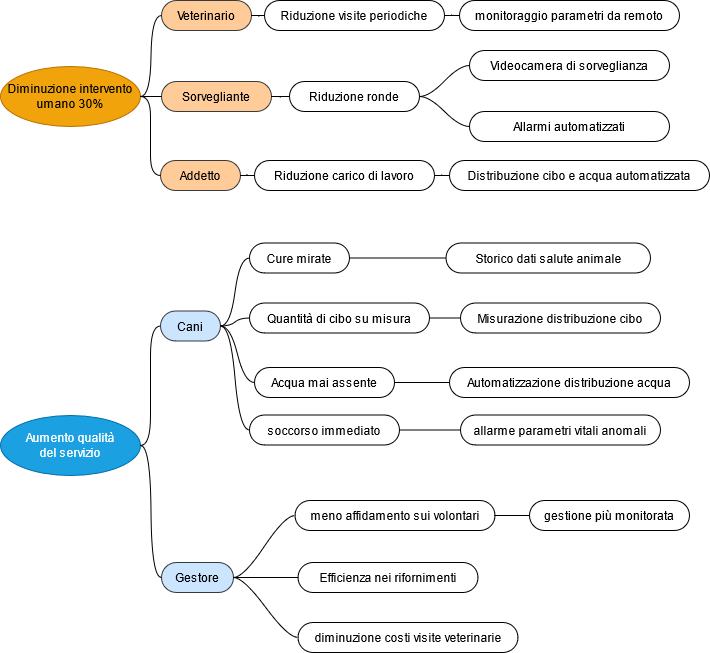
\includegraphics[width=1\textwidth]{DrawIo/impactMap.png}
    \end{figure}

    Il risultato ha portato in evidenza i due principali obbiettivi di business, evidenziando in maniera chiara la loro suddivisione, e le relative operazioni per raggiungere i risultati attesi.
    
    Con una visone d'insieme leggermente più definita, ci siamo cimentati nella stesura delle \textbf{user stories}. Cercando di seguire i due requisiti di business individuati, sono state identificate le più calzanti user stories per ogni obiettivo  dell'\textbf{impact map}
    .
    Nel tentativo di formalizzare le informazioni ottenute abbiamo suddiviso, raccolto e identificato le principali entità presenti. Sono state utilizzate successivamente per la definizione degli \textbf{use case diagram} che ne descrivessero le operazioni fondamentali.

	La definizione delle user-stories ha portato naturalmente a indagare il significato di alcuni termini usati. Questo ha spinto subito allo sviluppo di un ubiquitous language per i vocaboli più importanti, che poi è stato continuamente raffinato durante i successivi meeting. 
	Nel prossimo capitolo viene analizzato questo processo. 
    
	\section{Definizione Ubiquitus language}	
	L'Ubiquitous Language deve essere espresso nel modello di dominio, infatti unisce le persone del team di progetto.
    Lo scopo è eliminare le imprecisioni e le contraddizioni degli esperti di dominio, non è infatti imposto da questi, ma raggiunto collaborativamente.
    L'Ubiquitous Language si evolve nel tempo, non è definito interamente in una sola riunione, i concetti spesso si aggiungono, vengono sviscerati e partecipano nella comprensione del dominio. Infatti quelli che non fanno parte dell'Ubiquitous Language devono essere rifiutati.
    
    %TABELLA UBIQUITOUS LANGUAGE
    \begin{figure}[ht]
        \caption{Tabella ubiquitous language}
        \centering
        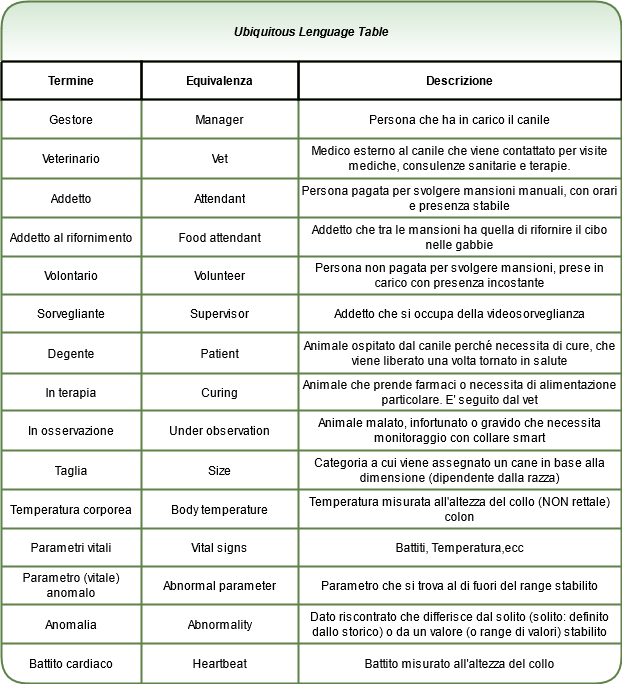
\includegraphics[width=1\textwidth]{DrawIo/ubiquitousLanguage.png}
    \end{figure}
